\documentclass[dvipdfmx]{jsarticle}

% 枠
\usepackage{fancybox}
\usepackage{ascmac}
% 色
\usepackage{color}
% 数式
\usepackage{amsmath}
\usepackage{amsfonts}
\usepackage{mathtools}
\usepackage{bm,physics}
\usepackage{siunitx}
\usepackage[thicklines]{cancel}
% 画像
\usepackage[dvipdfmx]{graphicx}
% \usepackage[draft]{graphicx} % 画像出力を枠だけにする.
\usepackage{here}
% グラフ
\usepackage{tikz}
\usetikzlibrary{
  intersections,
  calc,
  arrows.meta
}
% ソースコード
\usepackage{listings,jlisting}
\lstset{
  language=C++,
	stringstyle={\ttfamily},
	commentstyle={\ttfamily},
	basicstyle={\ttfamily},
	columns=fixed,
  frame={tb},
  breaklines=true,
  columns=[l]{fullflexible},
	backgroundcolor=\color[gray]{.90}, % pdfをコピペしたときに行番号を巻き込まないようにする.
  numbers=left, % 行数を表示したければonにする.
  xrightmargin=0em,
  xleftmargin=3em,
  numberstyle={\scriptsize},
  stepnumber=1,
  numbersep=1em,
	tabsize=2,
  lineskip=-0.5ex
}
% アンカー
\usepackage[dvipdfmx]{hyperref}
\usepackage{pxjahyper}
\hypersetup{
  setpagesize=false,
  bookmarksnumbered=true,
  bookmarksopen=true,
  colorlinks=true,
  linkcolor=black,
  citecolor=red,
  urlcolor=magenta
}
% 数式相互参照
\usepackage{cleveref}
\usepackage{autonum}
\numberwithin{equation}{subsection}

\begin{document}

% 表紙
\title{重力と熱流下における粒子集団の様相}
\author{理学部理学科物理学コース 学籍番号20S2035Y 山本 凜}
\date{\today}
\maketitle
\newpage
% 目次
\setcounter{tocdepth}{3}
\tableofcontents
\newpage
% 本文

% \chapter{実験モデル}
\section{系の設定}

2次元の気液共存系で, 質量$m$の粒子が$N$個存在することを考え, 系の上下には壁, 左右には周期境界条件を課す. また, 重力を$y$軸正の向きにかけて, 熱流を$y$軸負の向きに流す. この熱流は, 系の上下の領域にそれぞれ異なる温度を設定したlangevin熱浴を使用することによってかけることとし, NVT-MDシミュレーションを実行する. また, 各熱浴の$y$幅は$8\sigma$となるように設定する. (図\ref{fig:system})


\begin{figure}[H]
  \centering
  \caption{}
  \label{fig:system}
  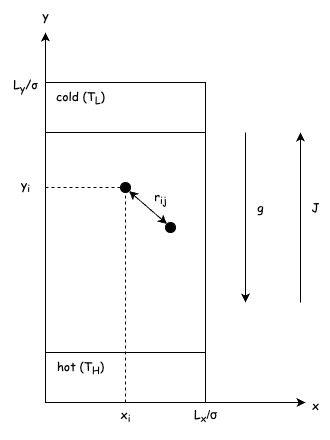
\includegraphics[scale=0.7]{image/system.jpg}
\end{figure}

\subsection{ハミルトニアン}

結論は, 

\begin{align}
  H(\Gamma; g)
  &= \sum_{i=1}^{N}
  \left[
    \frac{{\bm{p}_i}^2}{2m} 
    + \sum_{j > i}^{N}
      \tilde{\phi}_{\text{LJ}}^{\text{pair}}(r_{ij})
    + mgy_i
    + V^{\text{wall}} (y_i)
  \right] . \ \tag*{\eqref{Hamiltonian}} \\
  % \tilde{\phi}_{\text{LJ}}^{\text{pair}}(r ;r_{\text{cut}}^{\text{pair}}) 
  % &= \qty[4\varepsilon \qty{\qty(\frac{\sigma}{r})^{12} - \qty(\frac{\sigma}{r})^{6}} - 4\varepsilon \qty{\qty(\frac{\sigma}{r_{\text{cut}}^{\text{pair}}})^{12} - \qty(\frac{\sigma}{r_{\text{cut}}^{\text{pair}}})^{6}}]\theta \qty(r_{\text{cut}}^{\text{pair}}-r) \\
  % V^{\text{wall}} (y_;i) 
  % &= \tilde{\phi}_{\text{LJ}}^{\text{wall}}(y_i - 0;r_{\text{cut}}^{\text{wall}}) + \tilde{\phi}_{\text{LJ}}^{\text{wall}}(L_y - y_i;r_{\text{cut}}^{\text{wall}})
\end{align}

\subsubsection{粒子-粒子間相互作用ポテンシャル}

典型的な粒子間相互作用ポテンシャルとして, 12-6 Lennard-Jones Potential を採用する.

\begin{align}
  \phi_{\text{LJ}}^{\text{pair}}(r; \varepsilon, \sigma) = 4\varepsilon \qty[\qty(\frac{\sigma}{r})^{12} - \qty(\frac{\sigma}{r})^{6} ] \\
\end{align}

カットオフ長 $r_{\text{cut}}^{\text{pair}}=3\sigma$ とポテンシャルのシフトアップを考慮して

\begin{align}
  \tilde{\phi}_{\text{LJ}}^{\text{pair}}(r;r_{\text{cut}}^{\text{pair}}) = \qty{\phi_{\text{LJ}}^{\text{pair}}(r) - \phi_{\text{LJ}}^{\text{pair}}(r_{\text{cut}}^{\text{pair}})}\theta \qty(r_{\text{cut}}^{\text{pair}}-r) \\
\end{align}

% このポテンシャルを図示すると, 図\ref{fig:LJ-potential(pair)}のようになる.

% \begin{figure}[H]
%   \centering
%   \caption{}
%   \label{fig:LJ-potential(pair)}
%   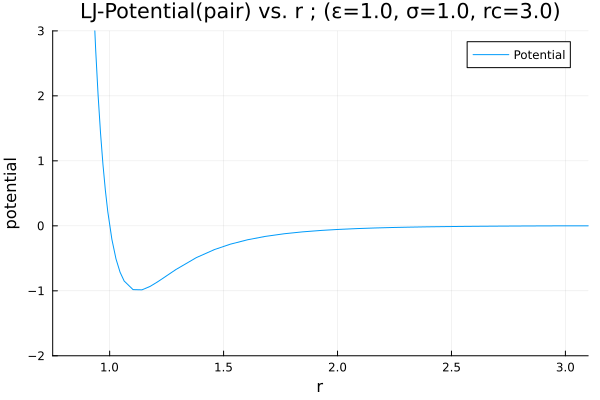
\includegraphics[scale=0.7]{image/LJ-Potential_pair_epsilon=1.0-sigma=1.0-rc=3.0.png}
% \end{figure}

\subsubsection{周期境界条件と最近接イメージ規約}

周期境界条件を考慮すると, 粒子-粒子間相互ポテンシャルの総計はまず以下のように書ける.

\begin{align}
  \sum_{n_x \in \mathbb{Z}} \sum_{i=1}^{N} \sum_{\substack{j=1 \\ (j \neq i \ \text{for} \ n_{x} = 0)}}^{N} \frac{1}{2} \phi_{\text{LJ}}^{\text{pair}}(|\bm{r}_i -(\bm{r}_j + L_x \bm{e}_x)|)
\end{align}

ここで, $n_x = 0$のオリジナルセルの中では, 同じ$i,\ j$ペアのポテンシャルエネルギーを2回足すことになるので, ポテンシャルを$1/2$している. その上で, $j = i$の場合は自分自身との相互作用になるため, これは除外する. $n_x \neq 0$の場合は, 粒子$j$はイメージ粒子となるので, $j=i$の場合も含める. この場合にもダブルカウントがあるので, ポテンシャルを$1/2$する.

\begin{figure}[H]
  \centering
  \caption{}
  \label{fig:system_periodic}
  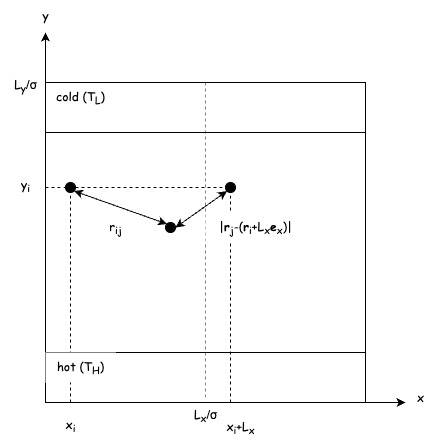
\includegraphics[scale=0.7]{image/system_periodic.jpg}
\end{figure}

また, 注目する系の粒子が常にオリジナルセルの中にとどまっているかのようにMD上で扱うには,

\begin{align}
  x_{i} = x_{i}' \mod L_{x}
\end{align}

のように,  飛び出した粒子の$x$座標$x_{i}'$を上式のように$x_i$にシフトすれば良い. しかし, 周期境界条件とセットにして, 最近接イメージ規約として, 粒子$i$がオリジナル粒子と各イメージ粒子の中で最も近い粒子$j$らとのみ相互作用をすることを考えると, 粒子間の相互ポテンシャルはより簡単に書けるようになる.

\begin{align}
  \sum_{i=1}^{N} \sum_{j > i}^{N} \phi_{\text{LJ}}^{\text{pair}} (r_{ij})
\end{align}





% また, 1次元の周期境界条件($x$軸両方向)を考慮するときには, 注目粒子$i$を$L_x$だけ$x$方向にずらして他の粒子$j$との相互作用を考えると適切に課すことができる.(式\eqref{eq:periodic}) ただし, これは$r_{\text{cut}}^{\text{pair}} < L_{x}/2$ であるような短いカットオフ長を選ぶことが前提である. (図3)

% \begin{align}
%   \sum_{i=1}^{N}\sum_{j=1}^{N}\tilde{\phi}_{\text{LJ}}^{\text{pair}}(|\bm{r}_j -(\bm{r}_i + L_x \bm{e}_x)|;r_{\text{cut}}^{\text{pair}}) \label{eq:periodic}
% \end{align}




\subsubsection{壁-粒子間相互作用ポテンシャル}


\begin{align}
  \phi_{\text{LJ}}^{\text{wall}}(r; \varepsilon^{\text{wall}}, \sigma^{\text{wall}}) = 4\varepsilon^{\text{wall}} \qty[\qty(\frac{\sigma^{\text{wall}}}{r})^{12} - \qty(\frac{\sigma^{\text{wall}}}{r})^{6} ] \\
\end{align}

パラメータは

\begin{align}
  \varepsilon^{\text{wall}} &= \qty(1.0 - \text{R}_\text{d}) \times \varepsilon \\
  \sigma^{\text{wall}} &= \qty(0.5 + \text{R}_\text{t}) \times \sigma \\
  r^{\text{wall}}_{\text{cut}} &= \qty(2^{1/6} + \text{R}_\text{a}) \times \sigma^{\text{wall}}
\end{align}



カットオフ長とシフトアップを考慮して



\begin{align}
  \tilde{\phi}_{\text{LJ}}^{\text{wall}}(r;r_{\text{cut}}^{\text{wall}}) = \qty{\phi_{\text{LJ}}^{\text{wall}}(r) - \phi_{\text{LJ}}^{\text{wall}}(r_{\text{cut}}^{\text{wall}})}\theta \qty(r_{\text{cut}}^{\text{wall}}-r) \\
\end{align}

このポテンシャルも図示したい. 

まず$r_{\text{attractive}} =0.0$, つまりカットオフ長 $r_{\text{cut}}^{\text{wall}}=0.5612\dots$のときは, 図\ref{fig:LJ-potential(wall)rc=0.5612}が示すようにWCAポテンシャルとなる.

\begin{figure}[H]
  \centering
  \caption{}
  \label{fig:LJ-potential(wall)rc=0.5612}
  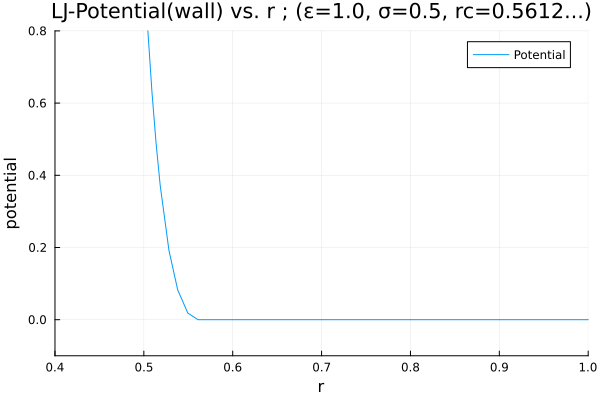
\includegraphics[scale=0.7]{image/LJ-Potential_wall_epsilon=1.0-sigma=0.5-rc=0.56.png}
\end{figure}

また, 参考のために, $r_{\text{cut}}^{\text{wall}}$ が$2^{1/6}\sigma^{\text{wall}}=0.5612\dots$から$3\sigma^{\text{wall}}=1.5$を超えるまで, $c_{\text{attractive}}$を0.0から2.0まで0.2ずつ増やした壁-粒子間の相互ポテンシャルの同時プロットを図示する.(図\ref{fig:LJ-Potential_wall_epsilon=1.0-sigma=0.5-rc}, 図\ref{fig:LJ-Potential_wall_epsilon=1.0-sigma=0.5-rc_zoom})

\begin{figure}[H]
  \centering
  \caption{}
  \label{fig:LJ-Potential_wall_epsilon=1.0-sigma=0.5-rc}
  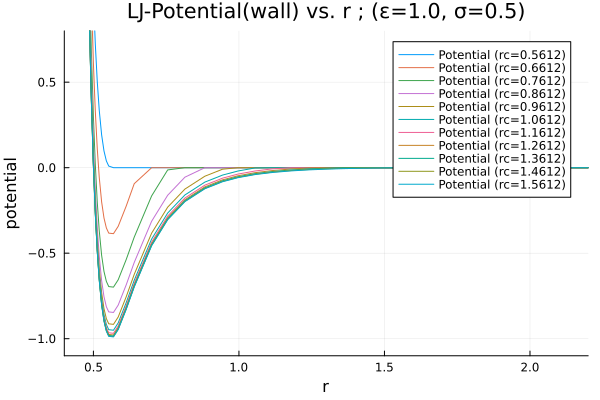
\includegraphics[scale=0.7]{image/LJ-Potential_wall_epsilon=1.0-sigma=0.5-rc.png}  
\end{figure}
\begin{figure}[H]
  \centering
  \caption{zoom}
  \label{fig:LJ-Potential_wall_epsilon=1.0-sigma=0.5-rc_zoom}
  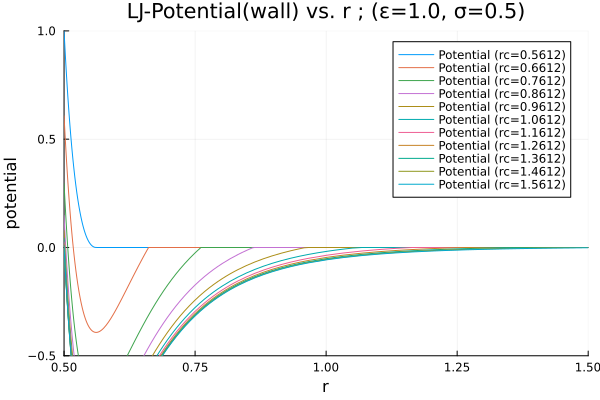
\includegraphics[scale=0.7]{image/LJ-Potential_wall_epsilon=1.0-sigma=0.5-rc_zoom.png}  
\end{figure}

図\ref{fig:LJ-Potential_wall_epsilon=1.0-sigma=0.5-rc_zoom}からもわかるように, $r = r_{\text{cut}}^{\text{wall}}$となるときには微分不可能であることには留意する必要がある.

このことから, 壁ポテンシャルは

\begin{align}
  V^{\text{wall}}(y; L_y) &= \tilde{\phi}_{\text{LJ}}^{\text{wall}}(y;r_{\text{cut}}^{\text{wall}}) + \tilde{\phi}_{\text{LJ}}^{\text{wall}}(L_y - y;r_{\text{cut}}^{\text{wall}})
\end{align}

周期境界条件を考慮した系のハミルトニアンは以下のように書き表せる.

\begin{align}
  \label{Hamiltonian}
    H(\Gamma; g)
    &= \sum_{i=1}^{N}
    \left[
      \frac{{\bm{p}_i}^2}{2m} 
      + \sum_{j > i}^{N}
        \tilde{\phi}_{\text{LJ}}^{\text{pair}}(r_{ij})
      + mgy_i +V^{\text{wall}}(y_i)
    \right]
\end{align}



\subsection{熱流}

langevin熱浴に侵入した粒子に対しては, brownian 動力学計算を実行する(\url{https://docs.lammps.org/fix_langevin.html}). その粒子$i$にはたらく力$\bm{F}_i$はLAMMPSのドキュメントに則った形式だと以下のように書き表せる.

\begin{align}
  \bm{F}_i &= \bm{F}_i^c + \bm{F}_i^f + \bm{F}_i^r \\
  \bm{F}_i^c &= - \bm{\nabla} 
  \left[
    \sum_{j > i}^{N}
        \tilde{\phi}_{\text{LJ}}^{\text{pair}}(r_{ij})
      + mgy_i +V^{\text{wall}}(y_i)
  \right]  \\
  \bm{F}_i^f &= -\frac{m_i}{\text{damp}}\bm{v}_i \\
  F_i^r &\propto \sqrt{\frac{k_\text{B} Tm_i}{dt \text{damp}}}
\end{align}

それぞれの力の説明を記す.

\begin{itemize}
  \item $\bm{F}^c$; ポテンシャルを介して計算される力
  \item $\bm{F}^f$; 摩擦力
  \item $\bm{F}^r$; ランダム力
\end{itemize}

\subsection{温度制御}


2d kinetic temperature

\begin{align}
  T \equiv \frac{1}{Nk_{\text{B}}}\sum_{i=1}^{N} \frac{1}{2}m_i v_{i}^2
\end{align}

粒子$i$が熱浴に侵入すると, その粒子の運動はランジュバン方程式に従う. 侵入していないときは, $\gamma = 0$になり, 正準方程式に等しくなる.

\begin{align}
  \dot{\bm{r}_i} &= \pdv{H}{\bm{p}_i} \\
  \dot{\bm{p}_i} &= - \pdv{H}{\bm{r}_i} - \gamma \dot{\bm{r}_i} + \sqrt{2 \gamma k_{\text{B}}T_{\nu}}\bm{\xi}_i (t) \\
  \expval{\xi_{i}^{a}(t)} &= 0 \\
  \expval{\xi_{i}^{a}(t)\xi_{j}^{b}(t')} &= \delta_{i,j} \delta_{a,b}\delta (t-t') \\
\end{align}

\begin{align}
  \gamma(y_i) &= 1. \ T_{\nu}(y_i) = T_{\text{H}}. \ (0 < y_i < 8\sigma) \\
  \gamma(y_i) &= 1. \ T_{\nu}(y_i) = T_{\text{C}}. \ (L_y - 8\sigma < y_i < L_y) \\
  \gamma(y_i) &= 0. \ T_{\nu}(y_i) = T. \ (8\sigma < y_i < L_y - 8\sigma)
\end{align}

% 見覚えのある形にすると, 

% \begin{align}
%   \bm{F}_i^f &= -\frac{m_i}{\gamma}\bm{v}_i \\
%   F_i^r &\propto \sqrt{\frac{m_i D}{dt}}
% \end{align}

% となる.


% \section{数値実験}

% \subsection{濡れ壁}

% 壁-粒子間相互作用ポテンシャルにおけるカットオフ長$r_{\text{cut}}^{\text{wall}}$をWCAポテンシャルに相当するところよりも大きくすると, 粒子は壁からの斥力だけでなく引力も受けるようになる.

% ここで, 重心($Y_g=\text{CoM[2]}$)のゆらぎ(標準偏差$\sigma(Y_g)$)を見る.

% パラメータ

% \begin{itemize}

% \end{itemize}

% \begin{align}
%   \sigma (Y_g) &= \sqrt{\frac{1}{\text{d}}\sum_{i=1}^{\text{d}}\qty(Y_{g}^i + \bar{Y_g})^2}
% \end{align}


% \subsection{壁の厚み}

\newpage

\section{追実験}

雨が降るシミュレーションを再現したい. 壁を完全に濡らしていることを考えたいので, $\sigma^{\text{wall}}=1.0\neq 0.5$ とする.

また, 系の両端のポテンシャルエネルギー差$mgL_y$と運動エネルギー差$k_{\text{B}}\Delta T$の比を$\chi$として以下のようにする.

\begin{align}
  \chi \equiv \frac{k_{\text{B}}\Delta T}{mgL_{y}} = 1.265
\end{align}

\subsection{先行研究の設定}

重力をかけた状態で緩和するまでシミュレーションを行う.

\begin{itemize}
  \item $N = 5000$
  \item $\rho \sigma^2 = 0.4$
  \item $L_x / \sigma = 79.0\dots$
  \item $L_y / \sigma = 158.1\dots$
  \item $k_{\text{B}} T/\varepsilon = 4.3$
  \item $k_{\text{B}} \Delta T/\varepsilon = 0.0$
  \item $mg = 2.0 \times 10^{-4}$
  \item $\sim t \sqrt{\varepsilon / m \sigma^2} = 5.0 \times 10^{5}$
\end{itemize}

重力をかけた緩和後の系で, 熱浴の温度差を以下のようにつけて, 熱流を流して実行をする.

\begin{itemize}
  \item $\chi = k_{\text{B}}\Delta T / mg L_y = 1.265$
  \item $k_{\text{B}} \Delta T/\varepsilon = 0.04$
  \item $\sim t \sqrt{\varepsilon / m \sigma^2} = 5.0 \times 10^{5}$
\end{itemize}

% \subsection{実際にやってみた}


% \begin{itemize}
%   \item $N = 1250$
%   \item $L_x / \sigma = 39.5\dots$
%   \item $L_y / \sigma = 79.0\dots$
%   \item $k_{\text{B}} T / \varepsilon = 0.43$
%   \item $k_{\text{B}} \Delta T / \varepsilon = 0.04$
%   \item $mg = 2.0 \times 10^{-4}$
%   \item $\tau \sqrt{\varepsilon / m \sigma^2} = 4.5 \times 10^{2}$
%   \item $t \sqrt{\varepsilon / m \sigma^2} = 5.0 \times 10^{4}$
% \end{itemize}

% \begin{figure}[H]
%   \centering
%   \href{https://youtube.com/shorts/5dD1dH0l6Ug?feature=share}{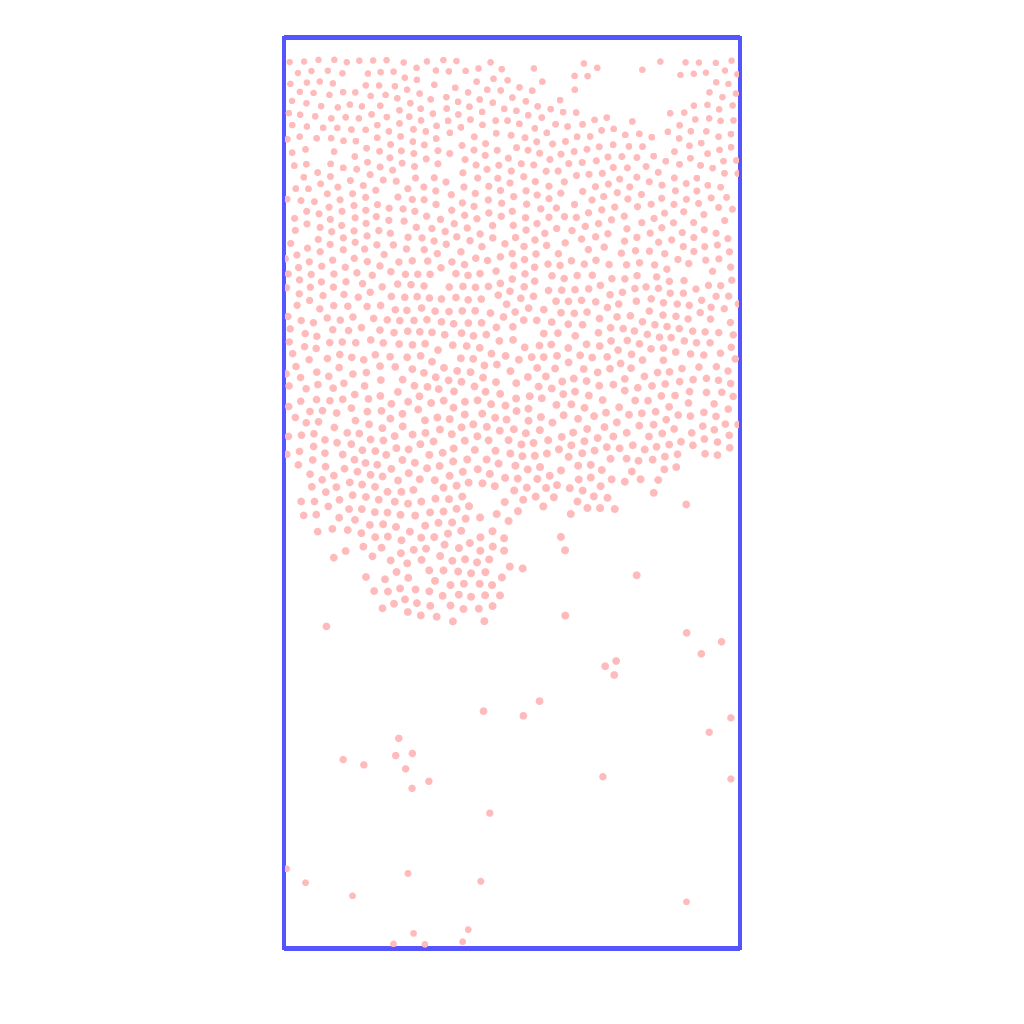
\includegraphics[scale=0.2]{image/rainAy50_rho0.4_T0.43_dT0.04_g0.0004_run1.0e7.png}}
%   \caption{rainAy50\_rho0.4\_T0.43\_dT0.04\_g0.0004\_run1.0e7}
% \end{figure}

% 系のサイズが小さいことで, 相対的に壁の引力の影響が大きくなってしまっていて, 粒子が落ちてこない現象が起きている可能性がある.

% \begin{itemize}
%   \item $N = 5000$
%   \item $L_x / \sigma = 79.0\dots$
%   \item $L_y / \sigma = 158.1\dots$
%   \item $k_{\text{B}} T / \varepsilon = 0.43$
%   \item $k_{\text{B}} \Delta T / \varepsilon = 0.04$
%   \item $mg = 2.0 \times 10^{-4}$
%   \item $\tau \sqrt{\varepsilon / m \sigma^2} = 4.5 \times 10^{2}$
%   \item $t \sqrt{\varepsilon / m \sigma^2} = 5.0 \times 10^{5}$
% \end{itemize}




% \begin{figure}[H]
%   \centering
%   \href{https://youtube.com/shorts/LvWMi7j88eQ?feature=share}{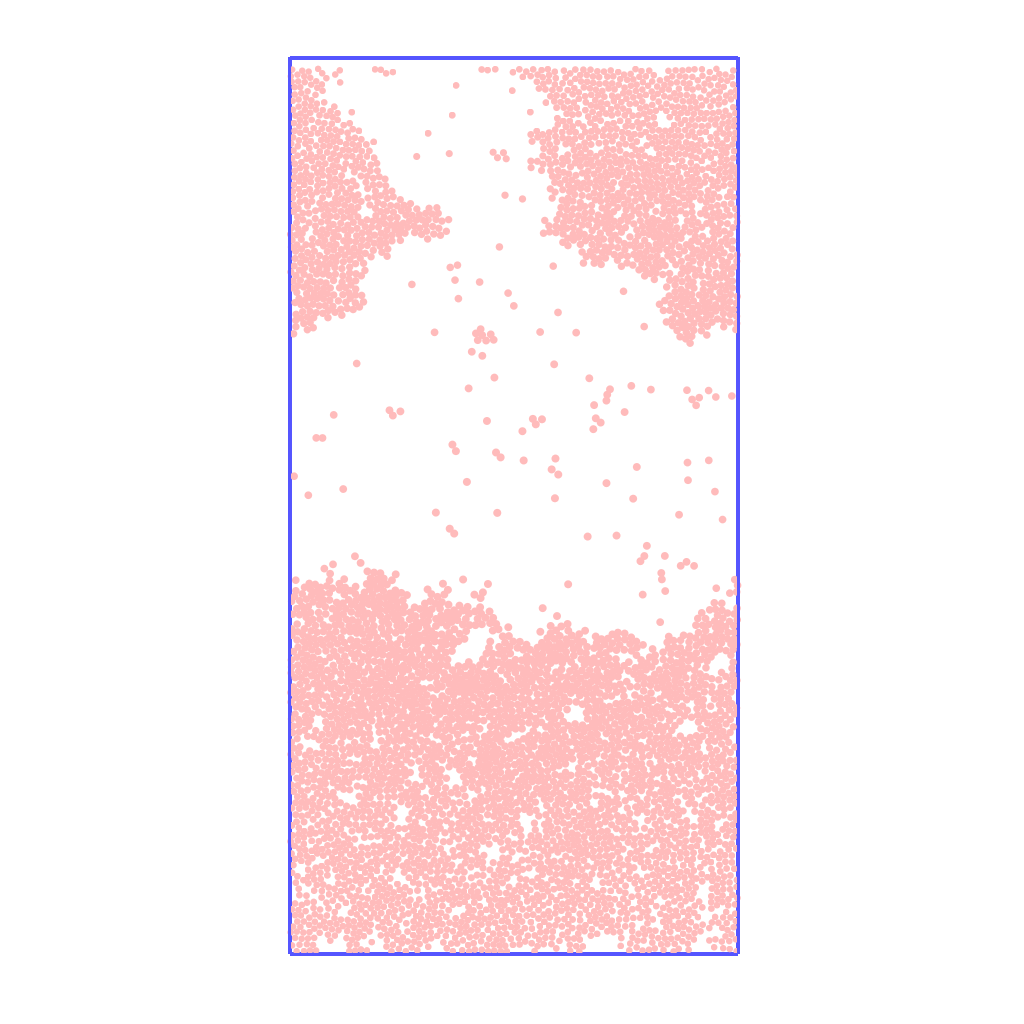
\includegraphics[scale=0.2]{image/rainAy100_rho0.4_T0.43_dT0.04_g0.0002_run1.0e8.png}}
%   \caption{Ay50\_rho0.4\_T0.43\_dT0.0\_g0.0\_run1.0e8}
% \end{figure}


% \begin{figure}[H]
%   \centering
%   \href{https://youtube.com/shorts/XPwz7CEhw_4?feature=share}{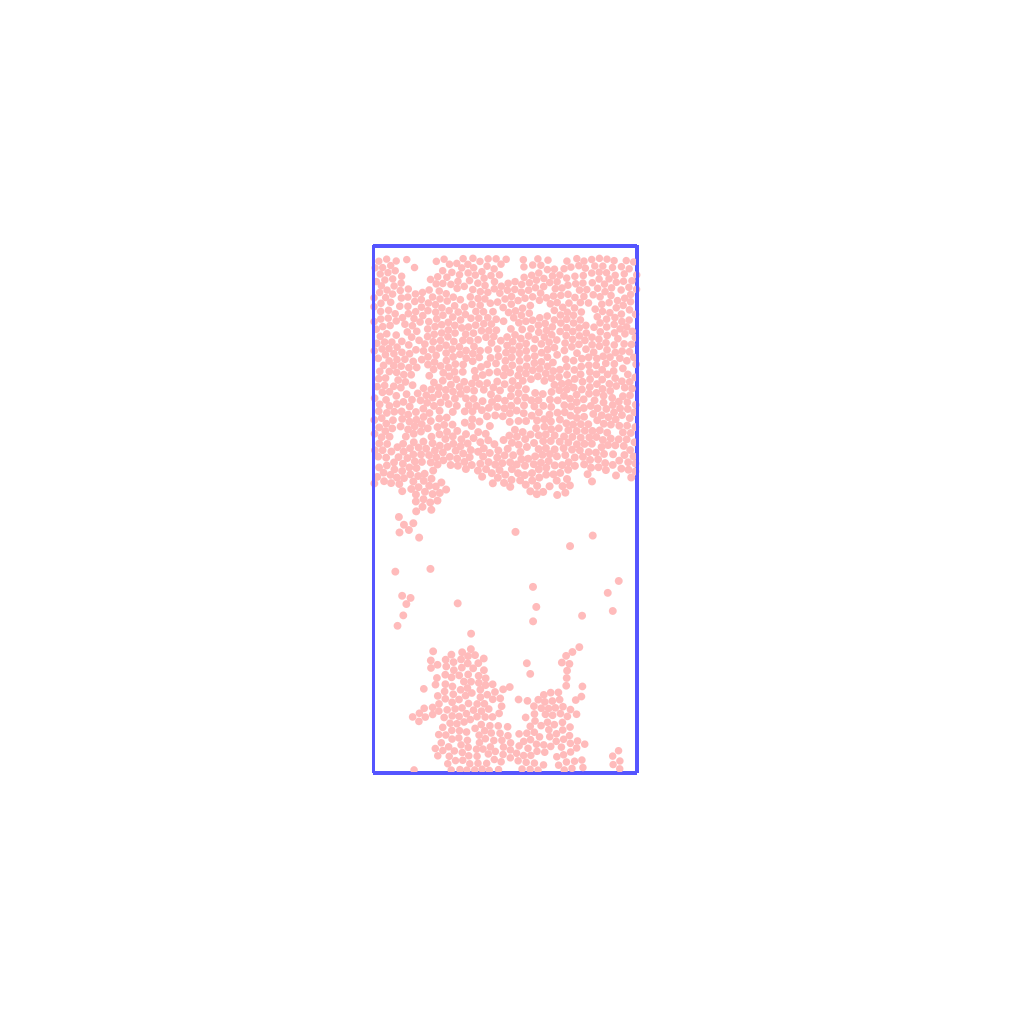
\includegraphics[scale=0.4]{image/Ay50_rho0.4_T0.43_dT0.0_g0.0_run1.0e7.png}}
%   \caption{Ay50\_rho0.4\_T0.43\_dT0.0\_g0.0\_run1.0e7}
% \end{figure}

% 重力と熱流を流さずに, 壁だけを濡らした.($r_{\text{cut}}^{\text{wall}}=3.0\sigma$)

% \begin{itemize}
%   \item $N = 1250$
%   \item $L_x / \sigma = 39.5\dots$
%   \item $L_y / \sigma = 79.0\dots$
%   \item $k_{\text{B}} T / \varepsilon = 0.43$
%   \item $k_{\text{B}} \Delta T / \varepsilon = 0.0$
%   \item $mg = 0.0$
%   \item $\tau \sqrt{\varepsilon / m \sigma^2} = 4.5 \times 10^{2}$
%   \item $t \sqrt{\varepsilon / m \sigma^2} = 5.0 \times 10^{4}$
% \end{itemize}

% \begin{figure}[H]
%   \centering
%   \href{https://youtube.com/shorts/XPwz7CEhw_4?feature=share}{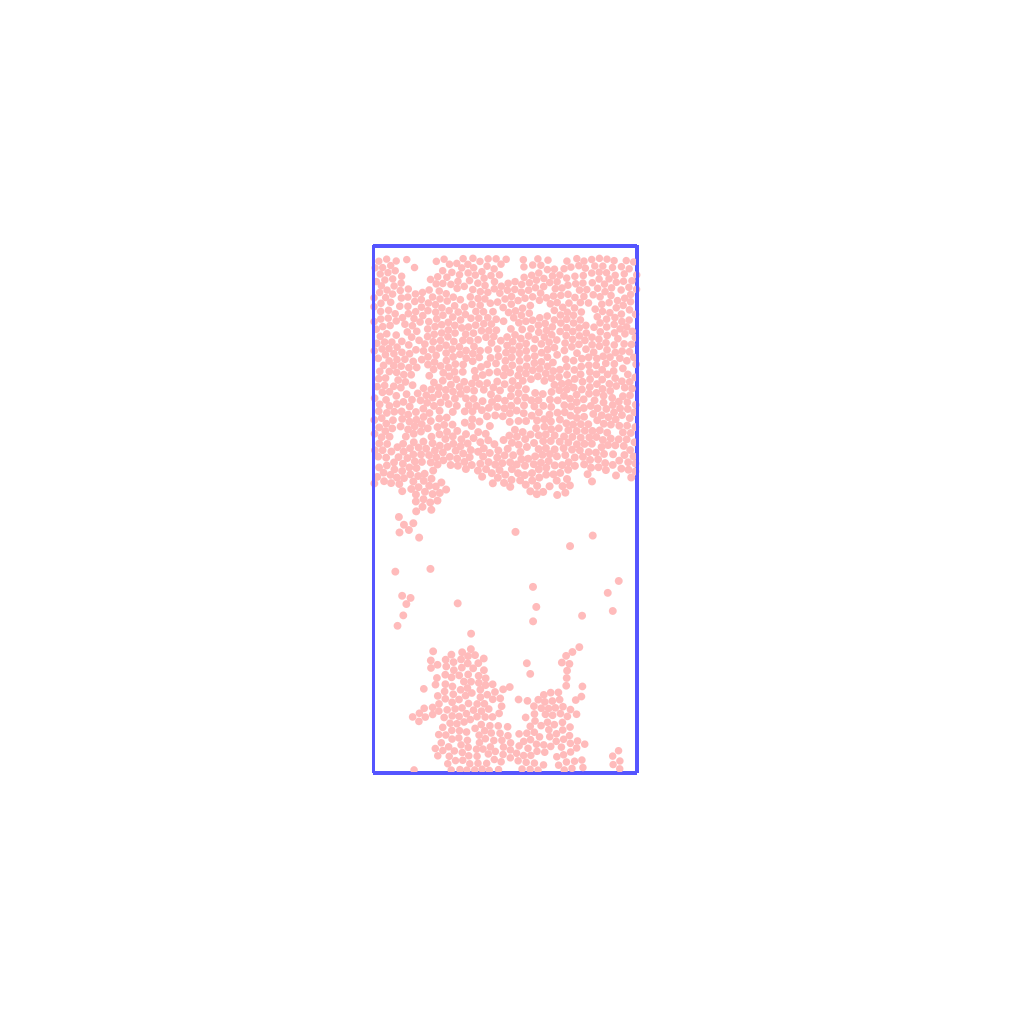
\includegraphics[scale=0.4]{image/Ay50_rho0.4_T0.43_dT0.0_g0.0_run1.0e7.png}}
%   \caption{Ay50\_rho0.4\_T0.43\_dT0.0\_g0.0\_run1.0e7}
% \end{figure}


% 熱流を流さずに, 重力をかけた.

% \begin{itemize}
%   \item $N = 1250$
%   \item $L_x / \sigma = 39.5\dots$
%   \item $L_y / \sigma = 79.0\dots$
%   \item $k_{\text{B}} T / \varepsilon = 0.43$
%   \item $k_{\text{B}} \Delta T / \varepsilon = 0.0$
%   \item $mg = 4.0 \times 10^{-4}$
%   \item $\tau \sqrt{\varepsilon / m \sigma^2} = 4.5 \times 10^{2}$
%   \item $t \sqrt{\varepsilon / m \sigma^2} = 5.0 \times 10^{4}$
% \end{itemize}

% \begin{figure}[H]
%   \centering
%   \href{https://youtube.com/shorts/OsQDscRtRgc?feature=share}{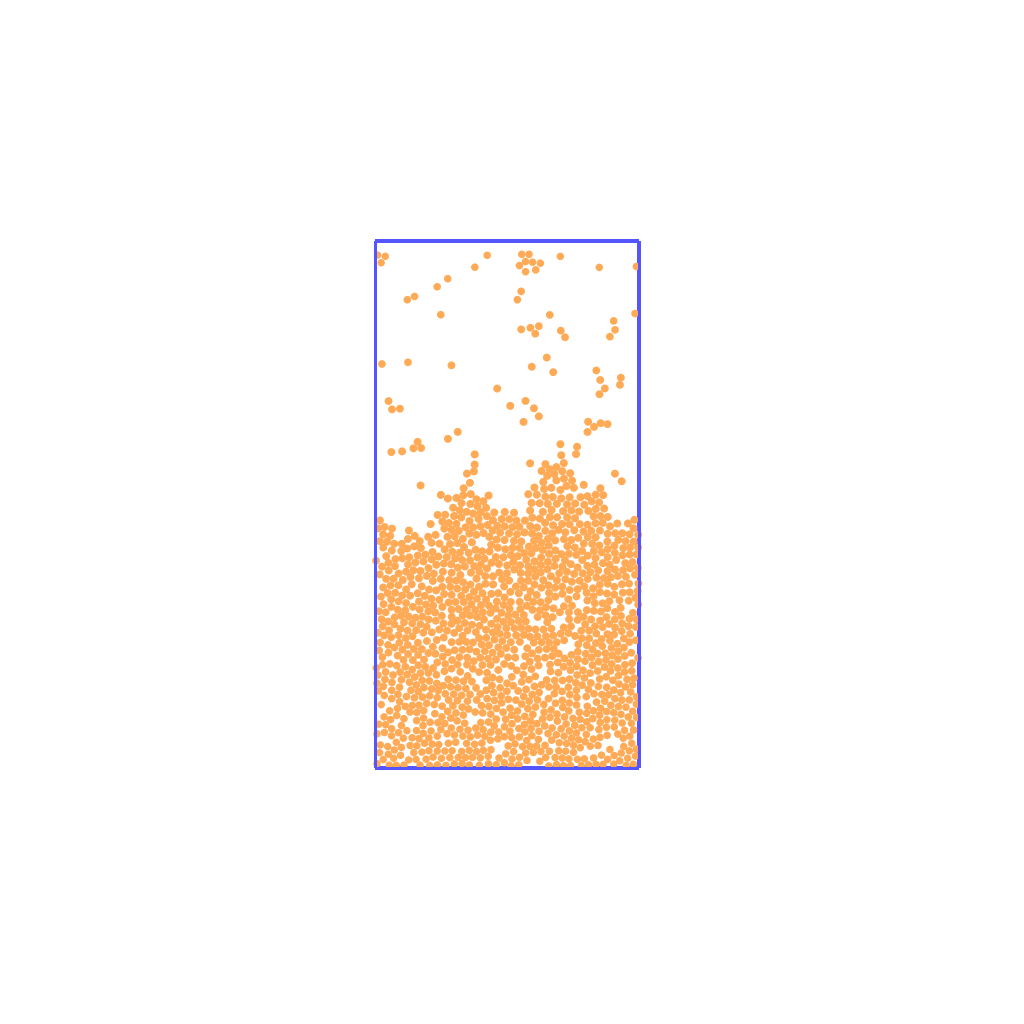
\includegraphics[scale=0.4]{image/Ay50_rho0.4_T0.43_dT0.0_g0.0004_run1.0e7.png}}
%   \caption{Ay50\_rho0.4\_T0.43\_dT0.0\_g0.0004\_run1.0e7}
% \end{figure}

% 重力と熱流をかけた.

% \begin{itemize}
%   \item $N = 1250$
%   \item $L_x / \sigma = 39.5\dots$
%   \item $L_y / \sigma = 79.0\dots$
%   \item $k_{\text{B}} T / \varepsilon = 0.43$
%   \item $k_{\text{B}} \Delta T / \varepsilon = 0.04$
%   \item $mg = 4.0 \times 10^{-4}$
%   \item $\tau \sqrt{\varepsilon / m \sigma^2} = 4.5 \times 10^{2}$
%   \item $t \sqrt{\varepsilon / m \sigma^2} = 5.0 \times 10^{4}$
% \end{itemize}

% \begin{figure}[H]
%   \centering
%   \href{https://youtube.com/shorts/muZ_mSa57xQ?feature=share}{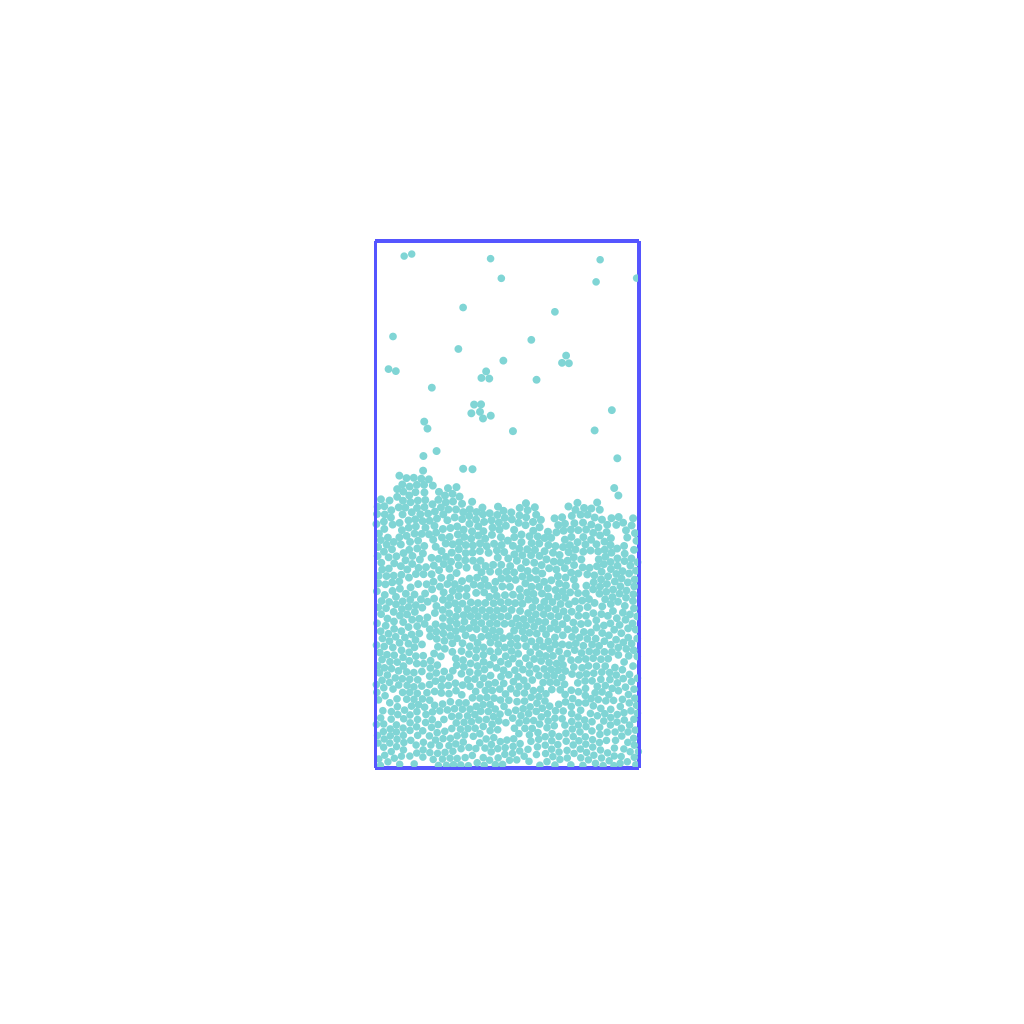
\includegraphics[scale=0.4]{image/Ay50_rho0.4_T0.43_dT0.04_g0.0004_run1.0e7.png}}
%   \caption{Ay50\_rho0.4\_T0.43\_dT0.04\_g0.0004\_run1.0e7}
% \end{figure}

\section{コレクション}

壁ポテンシャルまわりのパラメーターを3つ用意する.

\begin{align}
  \text{R}_\text{d} &: 乾き具合. \\
  \text{R}_\text{t} &: 壁の厚み. \\
  \text{R}_\text{a} &: 濡れ具合.
\end{align}

これに伴い, 壁-粒子間相互作用LJポテンシャルは以下のように書き表せるようになる.

\begin{align}
  \varepsilon^{\text{wall}} &= \qty(1.0 - \text{R}_\text{d}) \times \varepsilon \\
  \sigma^{\text{wall}} &= \qty(0.5 + \text{R}_\text{t}) \times \sigma \\
  r^{\text{wall}}_{\text{cut}} &= \qty(2^{1/6} + \text{R}_\text{a}) \times \sigma^{\text{wall}}
\end{align}

新たなパラメータ $(\text{R}_\text{d}, \text{R}_\text{t}, \text{R}_\text{a})$ を変えて, 壁-粒子間相互作用LJポテンシャルを変えたときにどのように粒子集団の様相が変化するかをみる. 以降の実験は基本的に以下のパラメータに近い値で行うものとする. 

\begin{itemize}
  \item $N = 1250$
  \item $\rho {\sigma}^2 = 0.4$
  \item $L_x / \sigma = 40$
  \item $L_y / \sigma = 80$
  \item $k_{\text{B}} T / \varepsilon = 0.43$
  \item $k_{\text{B}} \Delta T / \varepsilon = 0.04$
  \item $mg\sigma/\varepsilon = 4.0 \times 10^{-4}$
  \item $t_f \sqrt{\varepsilon / m \sigma^2} = 1.0 \times 10^{5}$
\end{itemize}

まずは, $(\text{R}_\text{d} = 0.0, \text{R}_\text{t} = 0.5, \text{R}_\text{a} = 3.0 - 2^{1/6})$ で実験を行う. これは, $(\varepsilon^{\text{wall}} = \varepsilon, \sigma^{\text{wall}} = \sigma, r^{\text{wall}}_{\text{cut}} = 3\sigma^{\text{wall}})$ に対応しているので, $\phi_{\text{LJ}} = \phi_{\text{LJ}}^{\text{wall}}$ ということになり, 追実験と同じ結果を得る. このときには, 壁の厚みが$0.5\sigma$で壁が十分に濡れていると考える.

\begin{figure}[H]
  \centering
  \href{https://youtu.be/fxn1mU1ZZFQ}{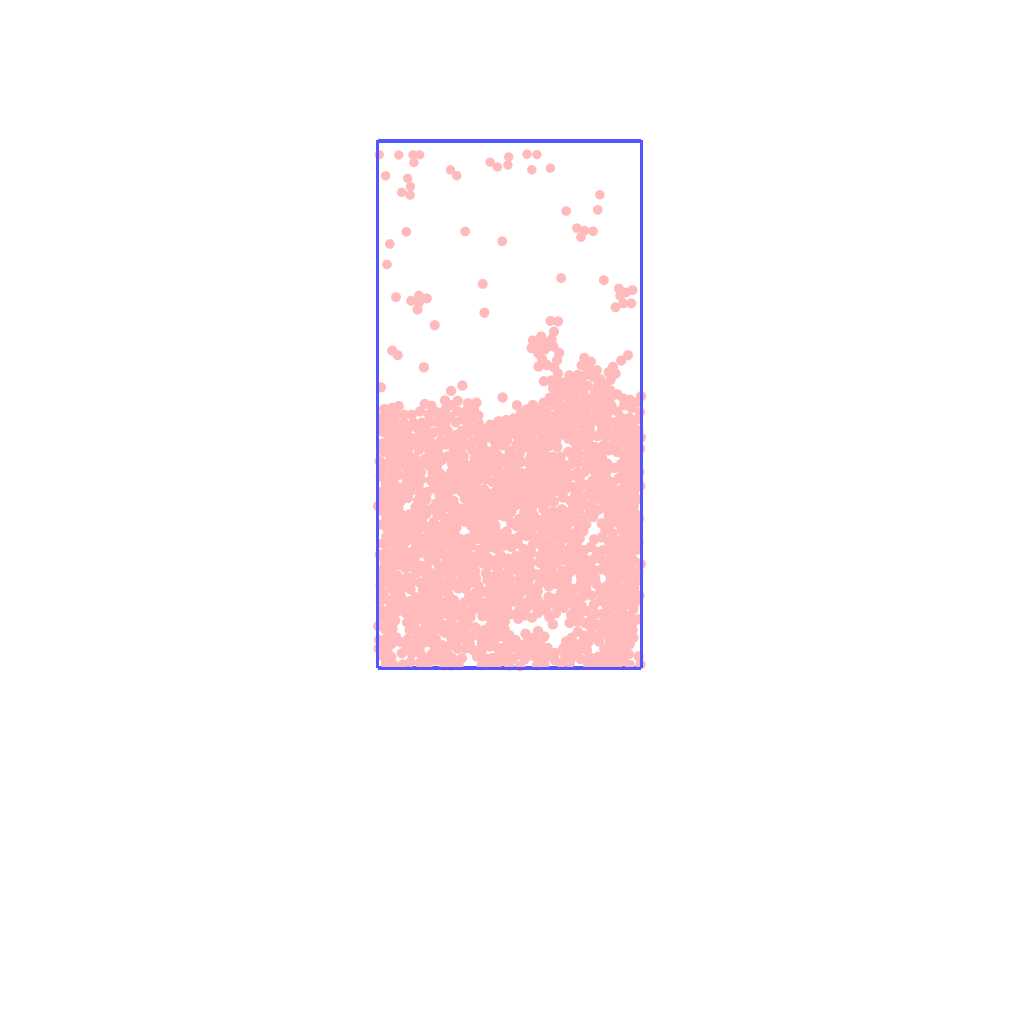
\includegraphics[scale=0.4]{image/2023-11-13T17:41:52.785__chi1.265_Ay50_rho0.4_T0.43_dT0.04_Rd0.0_Rt0.5_Ra1.877538_g0.0003999718779659611_run2.0e7_output.png}}
  \caption{Ay50\_rho0.4\_T0.43\_dT0.04\_Rd0.0\_Rt0.5\_Ra1.877538\_g0.0004\_run2.0e7}
\end{figure}

重心位置をスケーリングして, 時系列プロットすると,



\subsection{$\text{R}_\text{a}$, $\text{R}_\text{t}$}

$\text{R}_\text{a}$ を



\appendix
\section{ソースコード}

% \href{https://github.com/m-agnet/seminar.git}{GitHub}

\lstinputlisting[caption=in.vdw\_mod]{src/in.vdw2d_mod}
\lstinputlisting[caption=lammps\_modexe.jl]{src/lammps_modexe.jl}
\lstinputlisting[caption=LJpotential\_pair.jl]{src/LJpotential_pair.jl}
\lstinputlisting[caption=LJpotential\_wall.jl]{src/LJpotential_wall.jl}
\lstinputlisting[caption=iLJpotential\_wall\_rc.jl]{src/LJpotential_wall_rc.jl}


\end{document}